\documentclass[8pt]{beamer}
\usepackage[utf8]{inputenc}
\usepackage{xcolor}
\usepackage{colortbl}
\usepackage{epsfig}
% \usepackage{cancel}
\usepackage{ulem}
% \usepackage{threeparttable} % Joao Pela: 
\usepackage{amsmath}
\usepackage{hyperref}
\usepackage{appendixnumberbeamer}
% \usepackage{feynmp}         % For latex produced Feynman Diagrams

% Rule for feynmp diagrams to be considered graphics
% \DeclareGraphicsRule{*}{mps}{*}{}
% 
% % New compile sequence for feynmp
% \makeatletter
% \def\endfmffile{%
%   \fmfcmd{\p@rcent\space the end.^^J%
%           end.^^J%
%           endinput;}%
%   \if@fmfio
%     \immediate\closeout\@outfmf
%   \fi
%   \ifnum\pdfshellescape=\@ne
%     \immediate\write18{mpost \thefmffile}%
%   \fi}
% \makeatother

\usetheme{Madrid}

\author[J. Pela]{João Pela}
\title{L1 seeds for VBF Higgs to Invisible}
\institute[ICL]{Imperial College London}
\date{2016-04-14}

% The log drawn in the upper right corner.
\logo{\includegraphics[height=0.115\paperheight]{img/Logo_CMSICL.png}}

\begin{document}
\setlength{\unitlength}{1mm}

% ###################################################
\begin{frame}
  \titlepage
\end{frame}

% ###################################################
\begin{frame}{Today's presentation}
 
\begin{block}{Topics}
 
\begin{itemize}
  \item Comparison of L1T MET and MHT with/without inclusion of the HF.
  \item Optimisation study for possible seeds for VBF Higgs to Invisible analysis.
\end{itemize}
 
\end{block}

\end{frame}

% ###################################################
\begin{frame}{Samples and setup}

The results presented today use:
\begin{block}{Samples:}

\begin{itemize}
  \item Rate Calculations: ZeroBias - Run 259721 - PU 21-24
  \item Signal Efficiency: VBF Higgs to Invisible - PU Flat 10to25 25ns (TSG sample)
\end{itemize}

\end{block}

\begin{block}{Software setup:}
 
\begin{itemize}
  \item Emulator software tag: jetmet-update-forjoe-CMSSW\_8\_0\_2 (Jim Brooke's MET resolution fix)
  \item Ntuples produced with sums calculations with and without the inclusion of HF
\end{itemize}

\end{block}

\end{frame}

% ###################################################
\begin{frame}{L1 MET/MHT with/without HF}
 

\end{frame}

% ###################################################
\begin{frame}{L1 MET Rate vs Signal Efficiency curves}

\begin{columns}

\column[t]{0.45\linewidth}
\begin{block}{without HF}
 
\centering
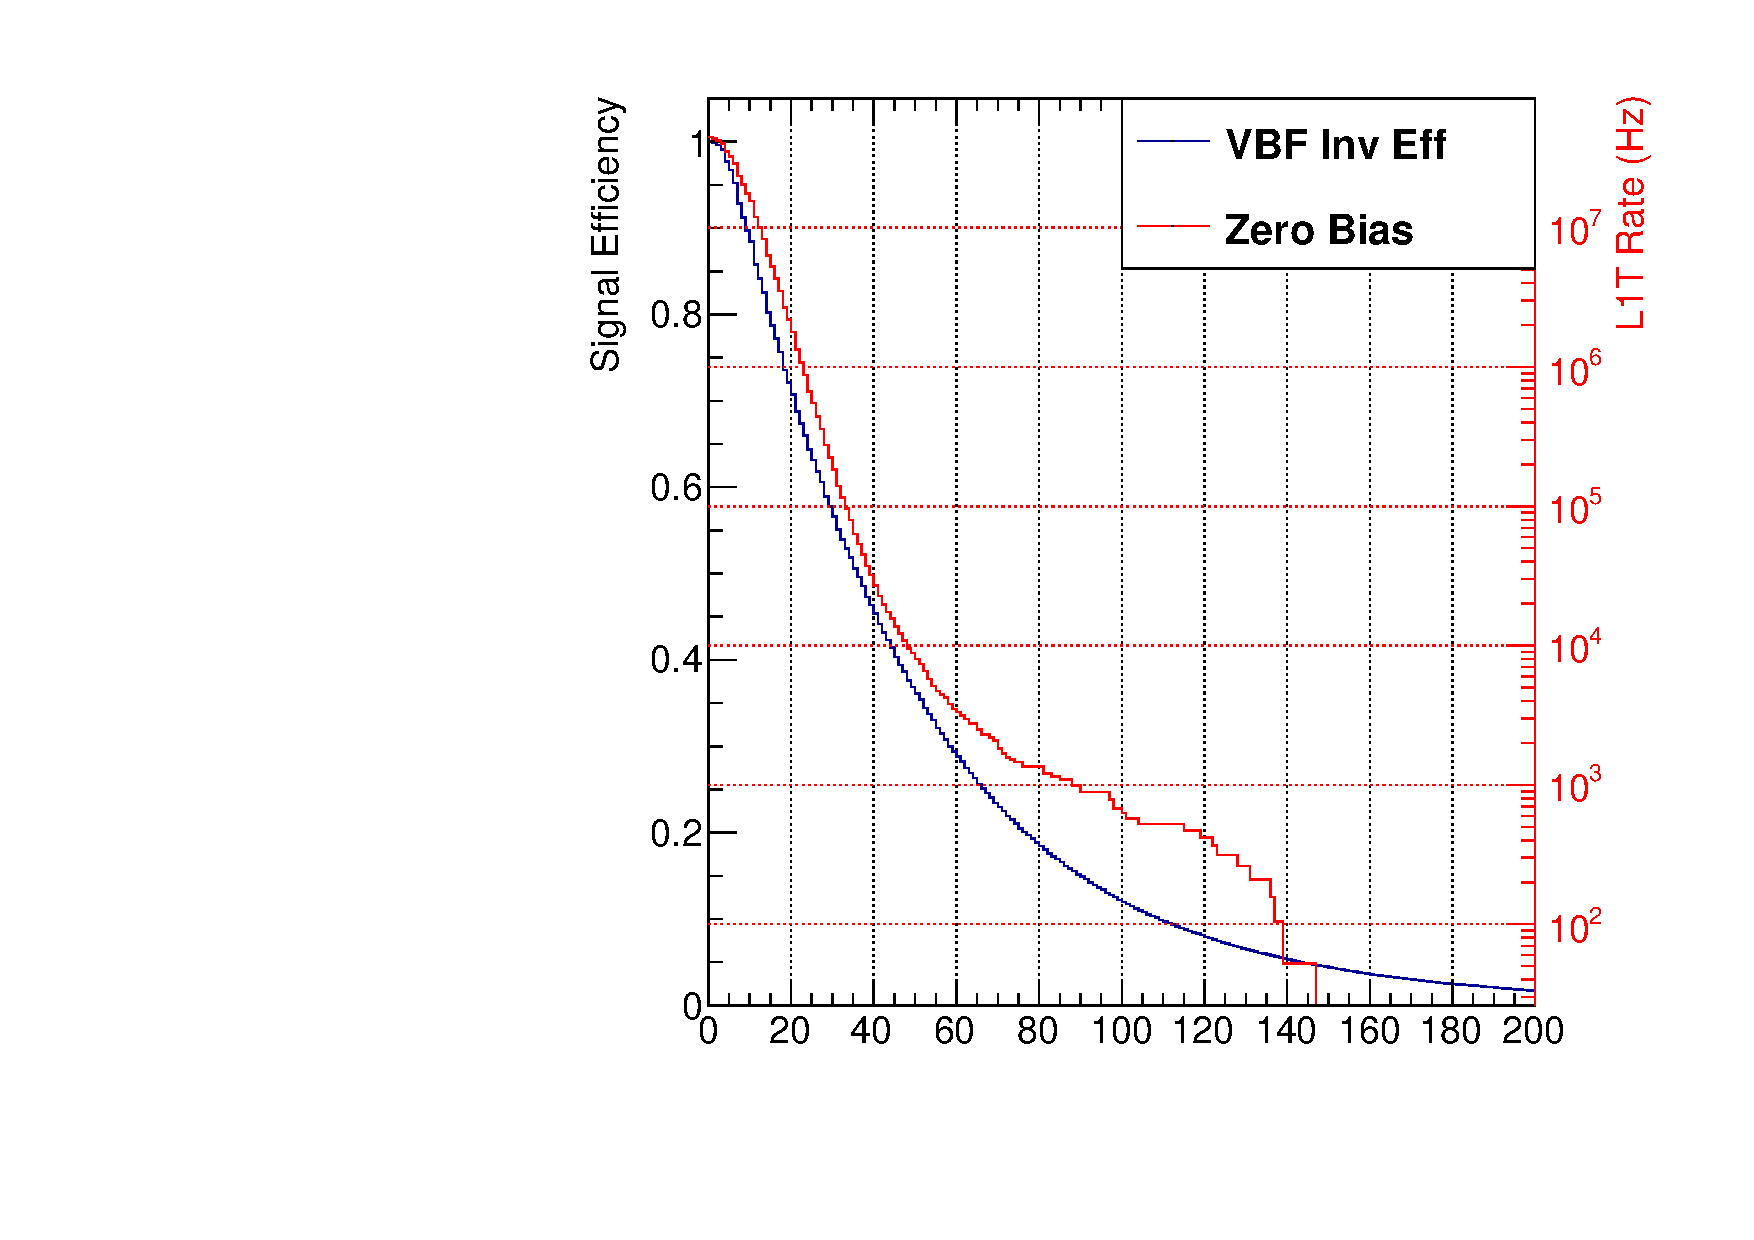
\includegraphics[width=\linewidth]{img/METRange3p0/L1TMet_Et.pdf}
 
\end{block}

\column[t]{0.45\linewidth}
\begin{block}{with HF}
 
\centering
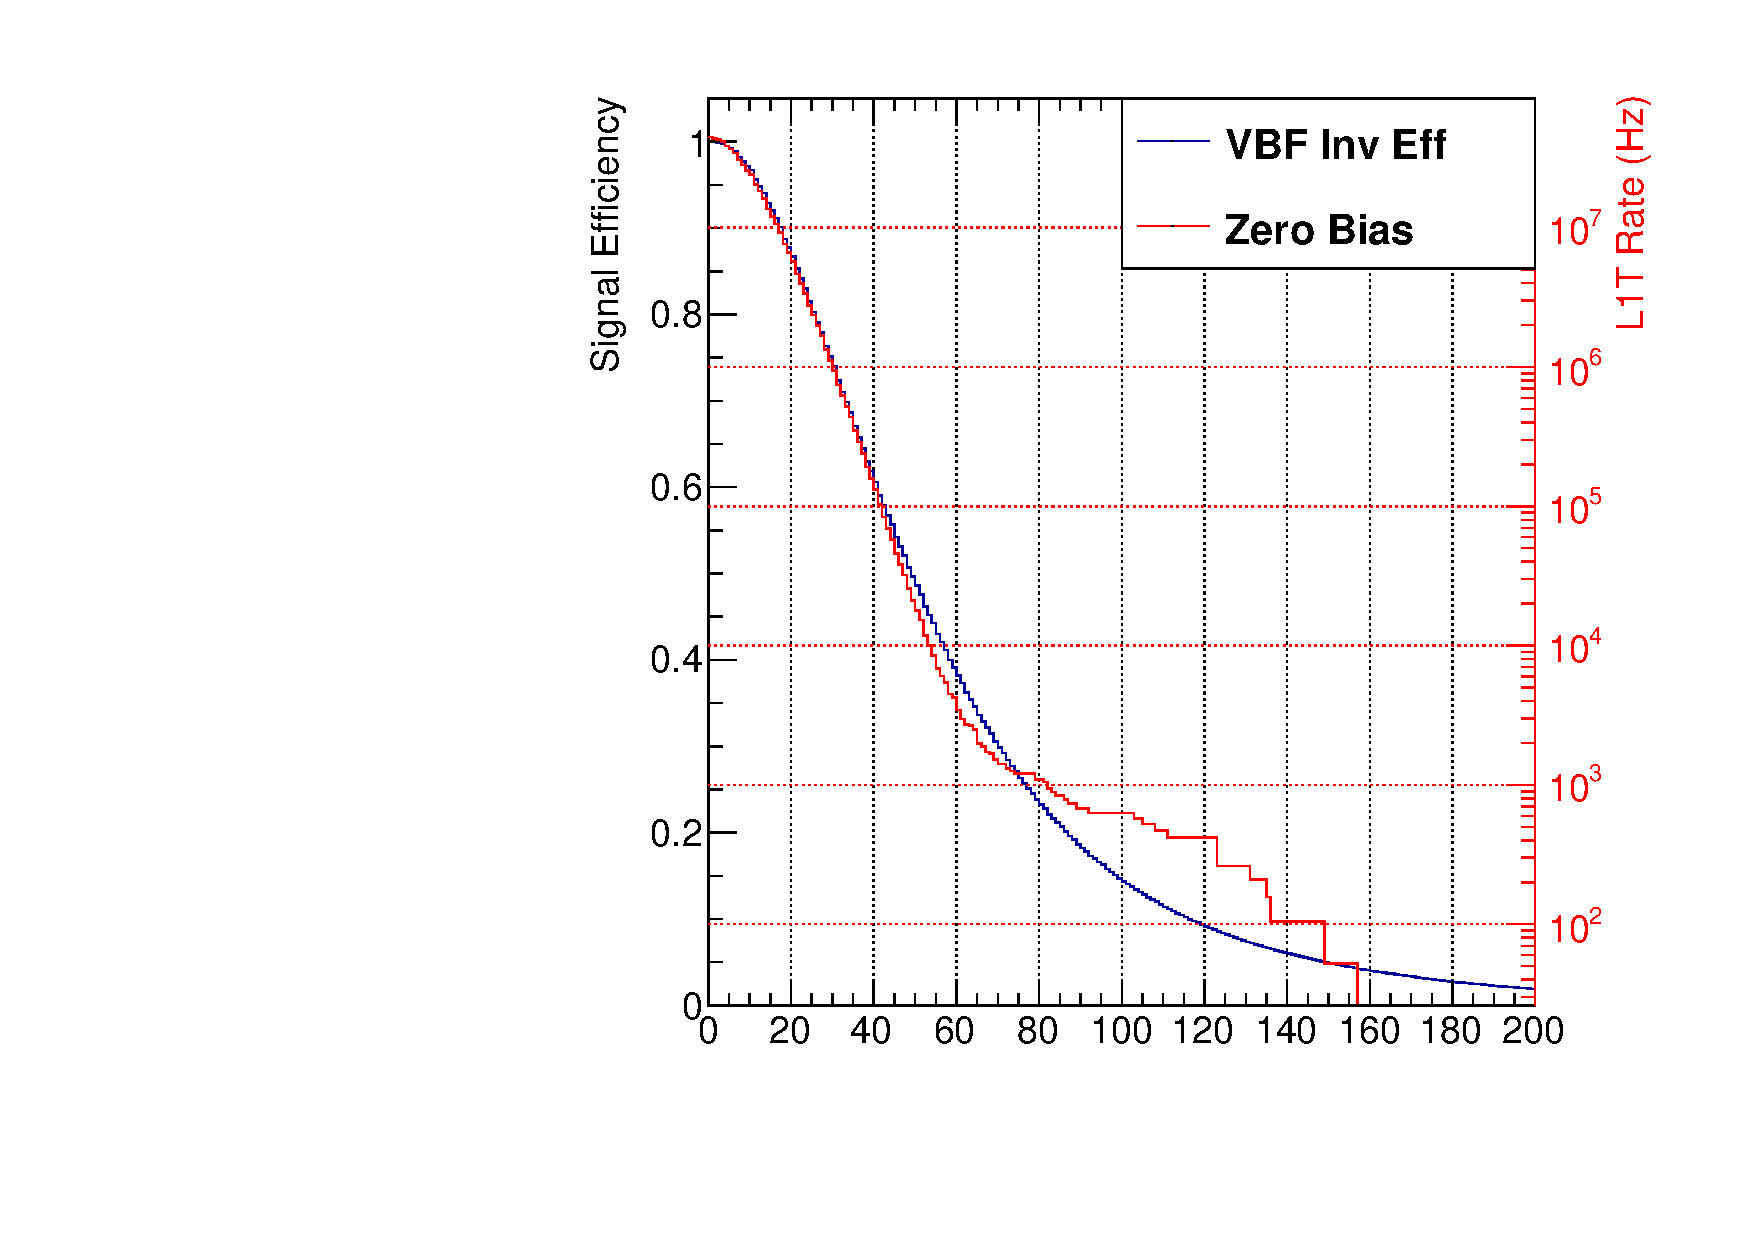
\includegraphics[width=\linewidth]{img/METRange5p0/L1TMet_Et.pdf}
 
\end{block}

\end{columns}
 
\end{frame}

% ###################################################
\begin{frame}{L1 MHT Rate vs Signal Efficiency curves}

\begin{columns}

\column[t]{0.45\linewidth}
\begin{block}{without HF}
 
\centering
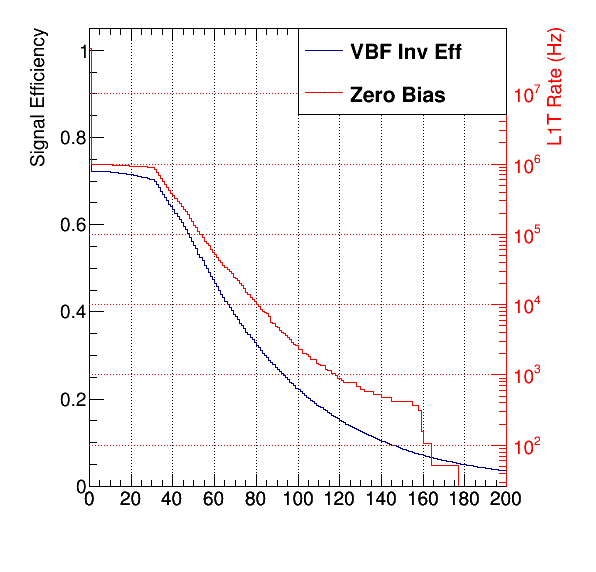
\includegraphics[width=\linewidth]{img/METRange3p0/L1TMHT_Et.png}
 
\end{block}

\column[t]{0.45\linewidth}
\begin{block}{with HF}
 
\centering
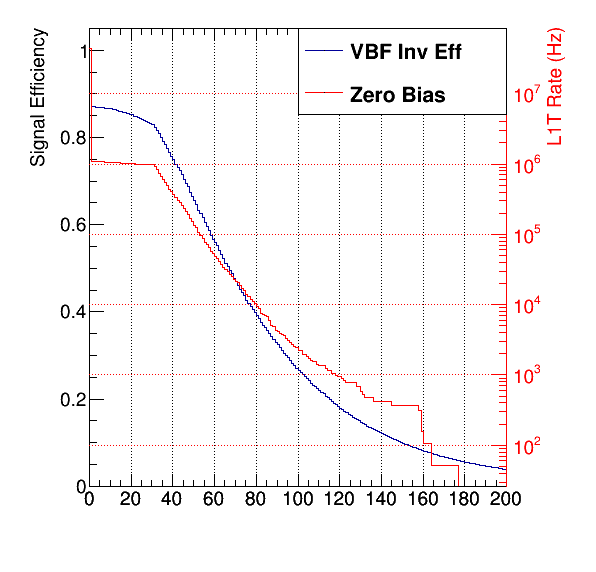
\includegraphics[width=\linewidth]{img/METRange5p0/L1TMHT_Et.png}
 
\end{block}

\end{columns}

\end{frame}

% ###################################################
\begin{frame}{L1T MET working points}
 
\begin{tabular}{|l|c|r||c|r|}
\hline
     & \multicolumn{2}{c||}{without HF} & \multicolumn{2}{c|}{with HF} \\
\hline \hline
Algo & Sig. Eff. & L1 Rate [Hz] & Sig. Eff. & L1 Rate [Hz] \\
\hline \hline
 MET40 & 0.4536 & 27648.7 & 0.6060 & 130663.0 \\
 MET50 & 0.3609 &  8604.6 & 0.4861 &  17494.9 \\
 MET60 & 0.2885 &  3606.4 & 0.3822 &   3227.8 \\
 MET70 & 0.2296 &  2024.6 & 0.2988 &   1355.7 \\
 MET80 & 0.1844 &  1455.2 & 0.2329 &   1097.5 \\
 MET90 & 0.1490 &   949.0 & 0.1821 &    710.1 \\
MET100 & 0.1197 &   632.7 & 0.1436 &    710.1 \\
MET110 & 0.0971 &   506.2 & 0.1141 &    516.5 \\
MET120 & 0.0793 &   379.6 & 0.0913 &    451.9 \\
MET130 & 0.0647 &   189.8 & 0.0734 &    258.2 \\
\hline
\end{tabular}
 
\end{frame}

% ###################################################
\begin{frame}{L1T MHT working points}

\begin{tabular}{|l|c|r||c|r|}
\hline
     & \multicolumn{2}{c||}{without HF} & \multicolumn{2}{c|}{with HF} \\
\hline \hline
Algo & Sig. Eff. & L1 Rate [Hz] & Sig. Eff. & L1 Rate [Hz] \\
\hline \hline
 MHT60 & 0.4660 & 52450.3 & 0.5594 & 49127.7 \\
 MHT70 & 0.3886 & 22966.8 & 0.4688 & 21368.3 \\
 MHT80 & 0.3236 & 10249.6 & 0.3908 &  9038.0 \\
 MHT90 & 0.2687 &  4618.7 & 0.3243 &  4196.2 \\
MHT100 & 0.2210 &  2404.2 & 0.2663 &  2324.0 \\
MHT110 & 0.1828 &  1518.5 & 0.2195 &  1420.3 \\
MHT120 & 0.1510 &   949.0 & 0.1792 &   903.8 \\
MHT130 & 0.1250 &   632.7 & 0.1462 &   516.5 \\
MHT140 & 0.1034 &   442.9 & 0.1203 &   516.5 \\
\hline
\end{tabular}

\end{frame}

% ###################################################
\begin{frame}{Search for L1T seeds for the VBF Higgs to Tnvisible analysis}
 
\end{frame}

% ###################################################
\begin{frame}{Search Results}
 
\end{frame}

% ###################################################
\begin{frame}{Conclusions}
 
\end{frame}

% % ###################################################
% \begin{frame}{Seeds}
% 
% Lets review our HLT paths and their corresponding seeds:
% 
% \begin{block}{HLT Paths vs. Seeds}
%  
% \resizebox{\linewidth}{!}{
% \begin{tabular}{|l|l|}
% \hline
% HLT Path & Seeds \\ 
% \hline \hline
% HLT\_DiPFJet40PFMETnoMu65MJJ600VBFLeadingJets & L1\_ETM40 \\
% HLT\_DiPFJet40PFMETnoMu65MJJ800VBFAllJets     & L1\_ETM40 \\
% \hline \hline
% HLT\_DiJet20\_MJJ650\_AllJets\_DEta3p5\_HT120\_VBF & L1\_HTT200 OR L1\_HTT175 OR L1\_ETM40 OR L1\_ETM50 \\
% HLT\_DiJet30\_MJJ700\_AllJets\_DEta3p5\_VBF        & L1\_HTT200 OR L1\_HTT175 OR L1\_ETM40 OR L1\_ETM50 \\
% HLT\_DiJet35\_MJJ650\_AllJets\_DEta3p5\_VBF        & L1\_HTT200 OR L1\_HTT175 OR L1\_HTT150 OR L1\_ETM40 \\
% HLT\_DiJet35\_MJJ700\_AllJets\_DEta3p5\_VBF        & L1\_HTT200 OR L1\_HTT175 OR L1\_ETM40 \\
% HLT\_DiJet35\_MJJ750\_AllJets\_DEta3p5\_VBF        & L1\_HTT200 OR L1\_HTT175 OR L1\_ETM40 \\
% \hline
% \end{tabular}
% }
% 
% \end{block}
% 
% Even though we only use L1\_ETM seeded events parked data paths have L1\_HTT seeds too.
% 
% \end{frame}
% 
% % ###################################################
% \begin{frame}{}
% 
% \begin{block}{Efficiencies}
%  
% \resizebox{\linewidth}{!}{
% \begin{tabular}{|l|l|l|l|l|}
% \hline
% Trigger                                      & 8 $TeV$   & PU40bx50  & PU20bx25   & PU40bx25  \\
% \hline \hline
% L1\_ETM40                                     & -         & 0.526785  & 0.48077    & 0.498313  \\
% \hline \hline
% HLT\_DiPFJet40PFMETnoMu65MJJ600VBFLeadingJets & 0.104736  & 0.11675   & 0.107917   & 0.10923   \\
% HLT\_DiPFJet40PFMETnoMu65MJJ800VBFAllJets     & 0.0766837 & 0.0919718 & 0.0849935  & 0.0878568 \\
% HLT\_DiJet35MJJ650VBFAllJets                  & 0.12091   & 0.0792947 & 0.12493    & 0.119854  \\
% HLT\_DiJet35MJJ700VBFAllJets                  & 0.109952  & 0.0691848 & 0.114779   & 0.10998   \\
% HLT\_DiJet35MJJ750VBFAllJets                  & 0.100287  & 0.0620005 & 0.106152   & 0.102006  \\
% HLT\_DiJet20MJJ650VBFAllJetsHT120             & 0.129063  & 0.105392  & 0.149766   & 0.13758   \\
% HLT\_DiJet30MJJ700VBFAllJets                  & 0.120932  & 0.0775783 & 0.127966   & 0.125002  \\
% \hline
% \end{tabular}
% }
% 
% \end{block}
% 
% \end{frame}
% 
% % ###################################################
% \begin{frame}{L1T ETM}
% 
% \begin{columns}
% 
% \column[t]{0.45\linewidth}
% \begin{block}{L1T ETM}
%  
% \centering
% 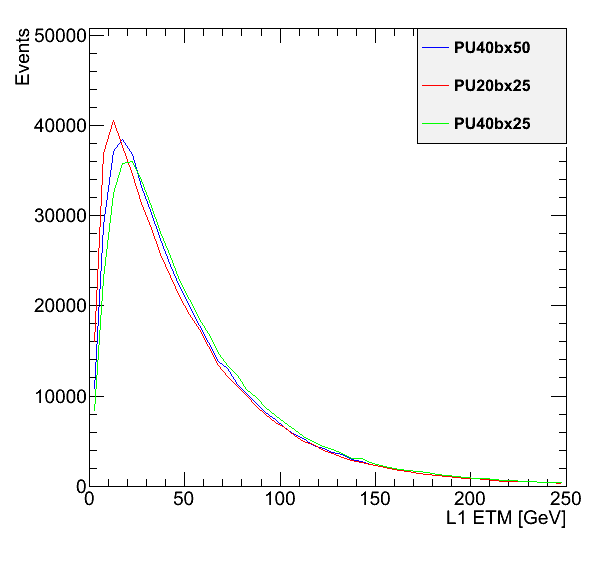
\includegraphics[width=\linewidth]{img/hL1ETM.png}
%  
% \end{block}
% 
% \column[t]{0.45\linewidth}
% \begin{block}{Sig. Eff. vs L1T ETM}
%  
% \centering
% 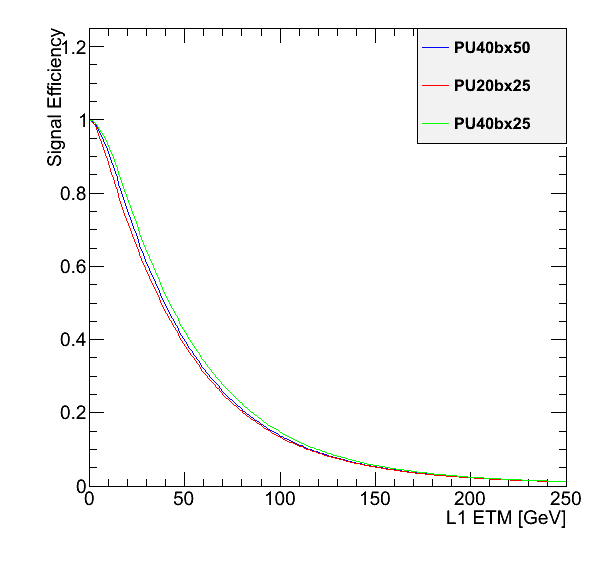
\includegraphics[width=\linewidth]{img/hEffL1ETM.png}
%  
% \end{block}
% 
% \end{columns}
% 
% \end{frame}
% 
% % ###################################################
% \begin{frame}{L1T HTT}
% 
% \begin{columns}
% 
% \column[t]{0.45\linewidth}
% \begin{block}{L1T HTT}
%  
% \centering
% 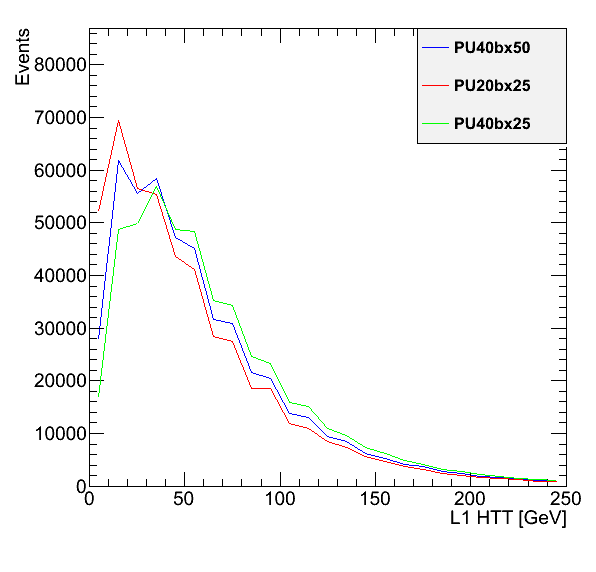
\includegraphics[width=\linewidth]{img/hL1HTT.png}
%  
% \end{block}
% 
% \column[t]{0.45\linewidth}
% \begin{block}{Sig. Eff. vs L1T HTT}
%  
% \centering
% 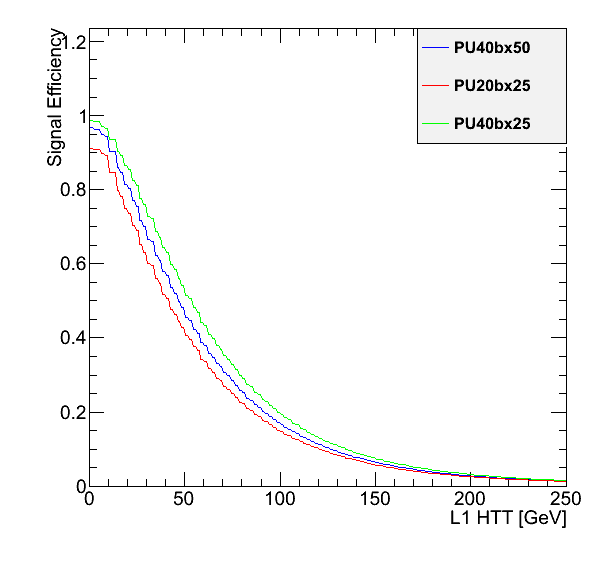
\includegraphics[width=\linewidth]{img/hEffL1HTT.png}
%  
% \end{block}
% 
% \end{columns}
% 
% L1 HTT is the sum of all L1 Jets and the kinks on the  plots are most likely due to two effects:
% \begin{itemize}
%   \item A L1 Jet seed need to have at least 5 $GeV$
%   \item A L1 Jet to be included in HTT needs to have at least least 10 $GeV$. 
% \end{itemize}
% 
% \end{frame}

% ###################################################
\begin{frame}{Summary and next steps}
 
\begin{block}{Summary:}
 
\begin{itemize}
  \item
\end{itemize}

\end{block}

\begin{block}{Next Steps:}
 
\begin{itemize}
  \item 
\end{itemize}
 
\end{block}

\end{frame}

\end{document}